% =============================================================================
% Section 10 — From Model to Clinic
% =============================================================================
\section{From Model to Clinic: What Survives, and What Humanity Gains}\label{sec:clinic}

\begin{objectives}
\begin{itemize}[leftmargin=*,itemsep=1pt,topsep=1pt]
  \item Trace which clinical conclusions survive the refutation of their supporting mechanism.
  \item Distinguish a therapeutic decision rule from the model once used to motivate it.
  \item State what formal methods contribute to medicine, and what they do not.
  \item Assess honestly what this book's programme offers and what it costs.
\end{itemize}
\end{objectives}

\subsection{The clinical fact}

Tumours carrying proofreading-domain \texttt{POLE} mutations are among the most
heavily mutated in oncology. A high tumour mutational burden (TMB) means many
neoantigens, which means a tumour visible to the immune system, which is why
such tumours respond well to checkpoint inhibition. Pembrolizumab is approved
for TMB-high solid tumours at a threshold of $\ge 10$ mutations per megabase.

This is a clinical fact, established by measuring mutation burden in patient
tumours and observing response. It does not depend on any model in this book.

\subsection{What the retracted model predicted}

Earlier editions of this material derived the TMB of a \texttt{P286R} tumour from
the stage-removal model. With $\gamma = 3/250$ and a wild-type burden of
$0.2$ mut/Mb, dropping from $m = 3$ to $m = 1$ multiplies by $1/\gamma^{2} =
62\,500/9$, giving
\begin{equation}\label{eq:tmbpred}
  \TMB_{\text{P286R}} \;=\; \tfrac{1}{5}\cdot\tfrac{62500}{9} \;=\; \tfrac{12500}{9} \;\approx\; 1388.9 \ \text{mut/Mb}.
\end{equation}
The arithmetic is exact, and Lean will confirm it. The mechanism it rests on was
refuted in Section~\ref{sec:refutation}.

So what is \eqref{eq:tmbpred} worth? As a prediction, nothing: it is the output
of a model we have shown to be false. As an illustration of a ratio computation,
it is fine. The honest handling is to keep it, label it, and never cite it as a
clinical quantity --- which is what Figure~\ref{fig:clinic}(a) does.

\begin{figure}[htbp]
  \centering
  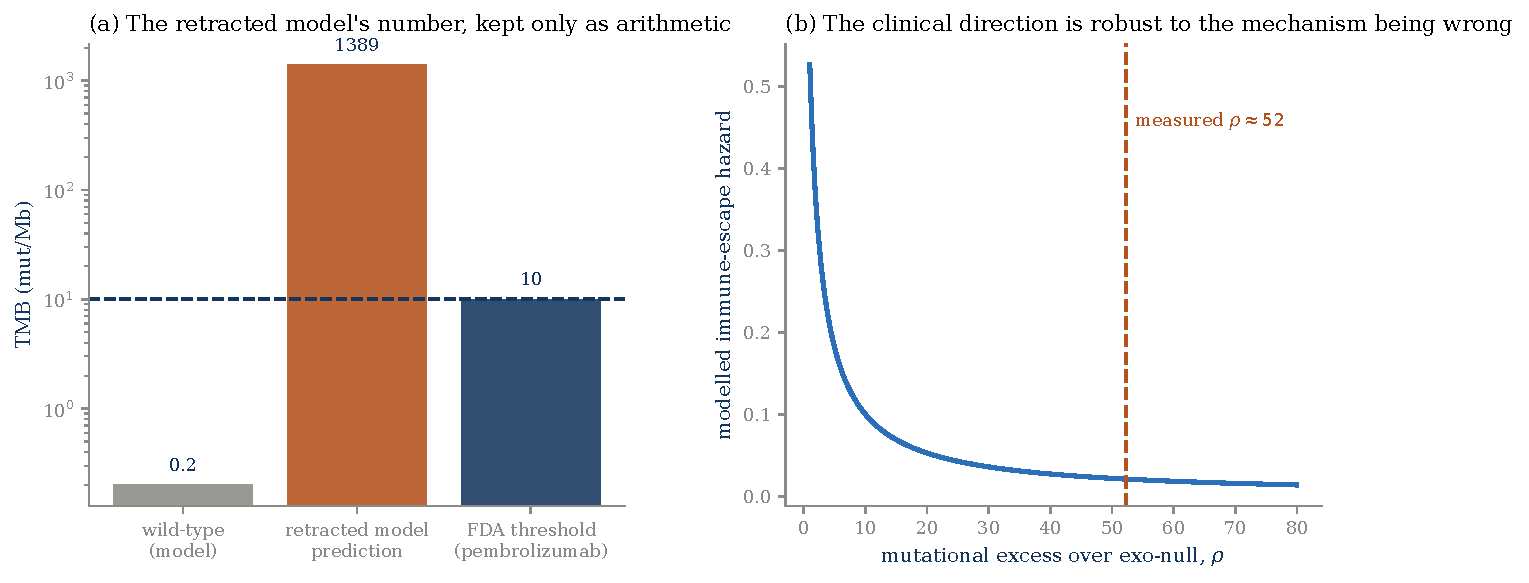
\includegraphics[width=\textwidth]{fig10_clinic.pdf}
  \caption{(a) The retracted model's prediction against the regulatory threshold,
  on a logarithmic axis. The bar is shown because deleting an error is worse
  pedagogy than displaying it, but it is arithmetic about a refuted model and not
  a claim about patients. (b) A modelled immune-escape hazard falling with
  mutational excess. The \emph{direction} of the clinical conclusion is robust:
  it does not depend on the mechanism that generates the excess.}
  \label{fig:clinic}
\end{figure}

\subsection{Why the clinical conclusion survives}

This is the most important distinction in the section, and it generalises well
beyond \texttt{POLE}.

The therapeutic decision rule is: \emph{measure TMB; if it exceeds $10$ mut/Mb,
consider checkpoint inhibition}. That rule takes TMB as an \emph{input}. It never
asks why the burden is high. A tumour mutated because proofreading failed, or
because repair was overwhelmed, or for a reason nobody has yet identified, enters
the rule identically.

The refuted model was never load-bearing for the clinic. It was an explanation
offered alongside a decision rule that measures the relevant quantity directly.
Refuting the explanation leaves the rule untouched.

\begin{remark}[The general pattern]
Clinical practice is often more robust than the mechanistic stories told around
it, because practice tends to measure the proximate quantity while stories
explain it. This is worth knowing in both directions. It means a refutation like
Section~\ref{sec:refutation}'s does not endanger patients --- but it also means a
mechanistic story that \emph{sounds} explanatory may be contributing nothing, and
its falsity may go unnoticed for years precisely because nothing downstream
depends on it. Ours went unnoticed for exactly that reason.
\end{remark}

\subsection{What formal methods are for in medicine}

It would be easy to end a book like this by claiming that machine-checked proof
will make biomedical science reliable. That claim would be false, and this book's
own history refutes it: every theorem in the retracted material passed the axiom
gate. The proofs were correct. The biology was wrong.

What formalisation did contribute is narrower and real:

\begin{enumerate}[leftmargin=*,itemsep=2pt]
  \item \textbf{It forced the hypothesis to be stated.} ``P286R removes
        proofreading stages'' became Assumption~\ref{model:class}, with an
        explicit domain and explicit ranges.
  \item \textbf{It made the hypothesis checkable.} Once stated that precisely,
        PSR$_2$ followed --- and PSR$_2$ had no free parameters, so a single
        ratio could kill it.
  \item \textbf{It located the replacement.} Theorem~\ref{thm:forced} does not
        guess at an interaction with repair; it derives one from two
        measurements.
\end{enumerate}

The contribution is \emph{exposure}, not certainty. A vague mechanism survives
indefinitely because nothing can contradict it. A formalised one can be killed by
one number, and ours was.

\subsection{The benefit to humanity, stated carefully}

The honest version of the humanitarian claim is modest and, we think, more
valuable for being modest.

Mechanistic errors in biomedical literature are common and persistent. They
persist because mechanisms are usually stated loosely enough to accommodate
contrary data. The practice this book demonstrates --- state the mechanism as a
model class, prove what the class entails without fitting, compare against a
directly measured reference, and publish the refutation when it comes --- is
transferable to any mechanistic claim in biology. It requires no new technology.
It requires being willing to write down what you believe precisely enough that it
can be shown wrong, and then to say so when it is.

The direct benefit is one retracted mechanism and a sharper question about
mismatch repair. The indirect benefit, if the practice spreads, is a literature
in which fewer wrong mechanisms survive for a decade. We would rather claim that
than claim to have cured anything.

\begin{worked}[10.1: does the refutation change any patient's care?]
\textbf{Problem.} A clinician reads Section~\ref{sec:refutation} and asks whether
the management of a \texttt{POLE}-mutant tumour should change.

\textbf{Solution.} No. The decision rule depends on measured TMB, which is
unaffected by why the burden is high. No recommendation in this book alters
eligibility, dosing or monitoring.

What \emph{could} change in future is prediction. If the mechanism is an
interaction with mismatch repair (Section~\ref{sec:mmr}), then a tumour's MMR
status becomes relevant to how mutagenic a given \texttt{POLE} variant will be ---
which would matter for interpreting variants of uncertain significance before a
burden has accumulated. That is a research direction, not current practice, and
Exercise~10.4 asks you to design the study.
\end{worked}

\begin{exercise}
Using \eqref{eq:tmbpred}, verify that $\frac{1}{5}\cdot\frac{62500}{9} =
\frac{12500}{9}$ exactly, and state in one sentence why verifying this arithmetic
tells you nothing about whether a \texttt{POLE} tumour has that burden.
\end{exercise}

\begin{exercise}
The threshold rule uses $\ge 10$ mut/Mb. Explain why a decision rule with a sharp
threshold can be robust to large errors in a mechanistic model, but is sensitive
to systematic bias in the assay that measures TMB.
\end{exercise}

\begin{exercise}
List three claims from Sections~\ref{sec:proofreading}--\ref{sec:dnatop} that
would change if the stage-removal model were resurrected, and three that would
not. What distinguishes the two groups?
\end{exercise}

\begin{exercise}[(harder)]
Design a retrospective study testing whether MMR status modifies the
\texttt{POLE}-variant-to-TMB relationship. State the cohort, the stratification,
the outcome, and --- most importantly --- the result that would refute the
hypothesis of Section~\ref{sec:mmr}.
\end{exercise}

\begin{ledger}
\textbf{Measured:} the pembrolizumab TMB threshold ($\ge 10$ mut/Mb) is a
regulatory criterion, not a measurement of ours. \texttt{POLE}-mutant tumours are
hypermutated: established in the clinical literature, independent of this book. \\
\textbf{Assumed:} the immune-escape hazard curve in Figure~\ref{fig:clinic}(b) is
illustrative, with no parameter estimated from patient data. It is drawn to show
a direction, and should not be read quantitatively. \\
\textbf{Proved:} only the arithmetic of \eqref{eq:tmbpred}, which is a fact about
the retracted model and not about tumours. \\
\textbf{Open:} whether MMR status modifies the variant-to-burden relationship in
patients. This is the clinically consequential question the refutation opens,
and this book does not answer it.
\end{ledger}
